\documentclass[conference]{IEEEtran}
\usepackage{amsmath,amssymb}
\usepackage{graphicx}
\usepackage{booktabs}
\usepackage{multirow}
\usepackage{xcolor}
\usepackage{cite}
\usepackage[hidelinks]{hyperref}
\graphicspath{{../figures/}}

\begin{document}

\title{Inventory Demand Forecasting via Kalman Filtering\\and Global DeepAR Models: A Hybrid Approach\\
\large Phase 2 --- Deep Learning Evaluation (CSA332)}

\author{
\IEEEauthorblockN{Saumya, Harshvardhan, Shivansh, Krishiv, Harsha}
\IEEEauthorblockA{B.Tech CS\&AI / CS\&DS, Semester 5 --- Deep Learning (CSA332)}
}

\maketitle

\begin{abstract}
Retail inventory planning needs probabilistic demand forecasts for many products whose sales are sparse, censored by stockouts,
and sometimes have almost no history. We compare a \emph{local} Kalman filter, a tabular LightGBM baseline and a \emph{global}
deep probabilistic model (DeepAR: LSTM with a Negative Binomial likelihood) on 300 SKUs of the M5 data set, using a rolling-origin
backtest with three origins, a 28-day horizon and three random seeds. We also propose \emph{KF-DeepAR}, a hybrid that feeds the
Kalman filter's causal predictions and their uncertainty to DeepAR as input channels. Stockouts are detected causally and \emph{marked},
never imputed. DeepAR improves the pinball loss over the best Phase-1 model (LightGBM) by 1.8\% (0.395 vs.\ 0.402) and over the Kalman
filter by 5.1\%. KF-DeepAR obtains the lowest pinball loss overall (0.394), significantly better than every Phase-1 model and than a fixed
50/50 Kalman+DeepAR average, with lower seed variance than DeepAR; its overall gain over DeepAR is not statistically significant,
but it is the best model for cold-start SKUs. An ablation study over seven design choices shows that the count (Negative Binomial) likelihood is the single most important component (+4.8\% pinball loss when replaced by a Gaussian),
while the other choices change the loss by less than the seed-to-seed variation.
\end{abstract}

\begin{IEEEkeywords}
probabilistic forecasting, DeepAR, LSTM, Kalman filter, hybrid models, intermittent demand, M5
\end{IEEEkeywords}

%======================================================================
\section{Introduction}
Retailers must decide how much stock to hold for thousands of products. Under-forecasting causes stockouts and lost
sales; over-forecasting ties up capital. Because the cost of the two errors differs, a \emph{point} forecast is not
enough: inventory decisions need \emph{quantiles} (e.g.\ the 90th percentile of next month's demand).

Retail demand is hard to forecast: most products sell a few units per day or less (\emph{intermittent} demand), recorded
zeros can be \emph{stockouts} rather than no demand, and new products have almost no history (\emph{cold start}).
Two families of models address different parts of this problem. A \emph{local} state-space model such as the Kalman
filter~\cite{kalman1960} tracks each product's level and adapts quickly, but learns nothing from other products.
A \emph{global} deep network such as DeepAR~\cite{salinas2020deepar} is trained on all products at once and learns shared
seasonal patterns, but only sees a fixed context window.

Phase~1 of this project built the machine-learning baselines (seasonal naive, LightGBM, per-SKU Kalman filter).
In Phase~2 we add deep learning and contribute:
\begin{enumerate}
  \item a leak-free DL data pipeline for M5 with a \emph{causal} stockout detector that marks, rather than imputes, censored days;
  \item a from-scratch PyTorch implementation of DeepAR (LSTM + Negative Binomial likelihood, ancestral sampling);
  \item \textbf{KF-DeepAR}, a hybrid in which the Kalman filter's causal one-step and $h$-step predictions and their
        uncertainty are fed to DeepAR as input channels;
  \item a rolling-origin backtest with MAE, RMSE, WAPE, pinball loss and interval coverage, seed variance, a paired bootstrap
        test, a cold-start experiment and an ablation study of seven design choices.
\end{enumerate}
All code is in Jupyter notebooks; each notebook and each section of the shared library notebook has a named owner.

%======================================================================
\section{Deep Learning Literature Review}
\subsection{Recurrent networks and gating}
Recurrent networks process a sequence by updating a hidden state. Back-propagation through time multiplies one Jacobian per step,
so gradients vanish or explode over long sequences~\cite{pascanu2013difficulty}. The LSTM~\cite{hochreiter1997lstm} adds a cell state
updated \emph{additively} through forget/input gates, giving a near-constant gradient path; the GRU~\cite{cho2014gru} merges the gates
into an update and a reset gate with fewer parameters. Pascanu et al.~\cite{pascanu2013difficulty} also proposed gradient-norm clipping,
which we use. Regularisation follows standard practice~\cite{goodfellow2016dl,prince2023udl}: dropout~\cite{srivastava2014dropout} and
decoupled weight decay (AdamW)~\cite{loshchilov2019adamw,kingma2015adam}.

\subsection{Global probabilistic forecasters}
DeepAR~\cite{salinas2020deepar} trains one autoregressive LSTM on many related series, outputs the parameters of a likelihood
(Negative Binomial for counts) and forecasts by sampling paths; it handles scale differences by dividing by the context mean.
MQ-RNN~\cite{wen2017mqrnn} instead predicts several quantiles for all horizons directly with a quantile loss, avoiding sampling.
The Temporal Fusion Transformer~\cite{lim2021tft} replaces recurrence by attention and adds variable-selection networks for
interpretability. Montero-Manso and Hyndman~\cite{montero2021locality} show theoretically that a global model can be at least as
expressive as a set of local models and generalises better when individual series are short --- the motivation for global DL here.

\subsection{State-space models and hybrids}
The Kalman filter~\cite{kalman1960,durbin2012ssm} gives the optimal linear estimate of a latent state and its variance, handles missing
observations exactly and provides a likelihood for parameter estimation. Hybrids combine this with deep learning: ES-RNN~\cite{smyl2020esrnn},
winner of M4, normalises each series with per-series exponential-smoothing states and lets a global LSTM model the rest;
Deep State Space Models~\cite{rangapuram2018dssm} let an RNN output the parameters of a per-series linear-Gaussian SSM.
Recent selective SSMs such as Mamba~\cite{gu2023mamba} can be seen as learned, input-dependent versions of the same linear recurrence.
Classical forecast combination~\cite{bates1969combination} averages model outputs with fixed weights; we use it as a control for our hybrid.

\subsection{Retail and intermittent demand}
The M5 competition~\cite{makridakis2022m5} (Walmart, 42{,}840 series) found that global tree models (LightGBM~\cite{ke2017lightgbm})
and global neural networks clearly beat local statistical methods, and that exogenous calendar/price features matter.
Intermittent demand is categorised by the average inter-demand interval and the variability of non-zero sizes~\cite{syntetos2005categorization}.

\subsection{Evaluation}
Quantile forecasts are evaluated with the pinball loss~\cite{koenker1978quantile}, a strictly proper scoring rule~\cite{gneiting2007proper}.
Out-of-sample evaluation over several rolling forecast origins~\cite{tashman2000rolling,hyndman2021fpp3} avoids conclusions that depend on one test period.

%======================================================================
\section{Data and DL Dataset}
\subsection{Subset}
We use M5~\cite{makridakis2022m5} store CA\_1 and three departments with different behaviour: FOODS\_3 (high volume),
HOUSEHOLD\_1 and HOBBIES\_1 (sparse). 100 SKUs are sampled at random from each (seed 42), giving $N=300$ daily series over the last
$T=1000$ days (Aug.~2013--May~2016). Table~\ref{tab:segments} shows that most series are intermittent.

\begin{table}[t]
\centering
\caption{Syntetos--Boylan demand segments of the 300 SKUs (training period).}
\label{tab:segments}
\begin{tabular}{lcccc}
\toprule
Department & smooth & erratic & intermittent & lumpy\\
\midrule
FOODS\_3 & 17 & 4 & 51 & 28\\
HOUSEHOLD\_1 & 16 & 1 & 75 & 8\\
HOBBIES\_1 & 3 & 8 & 75 & 14\\
\midrule
Total & 36 & 13 & 201 & 50\\
\bottomrule
\end{tabular}
\end{table}

\subsection{Cleaning rules}
\textbf{Complete index.} Every (SKU, day) pair exists (asserted).
\textbf{Availability.} Weeks without a price mean the item is not on sale (e.g.\ not yet launched); those days, and the three Christmas
closures, are set to missing, not zero. 52 SKUs launch inside the window.
\textbf{Stockouts (mark, don't impute).} Under a Poisson model with rate $\lambda$ equal to the mean of the 56 days before a zero-run starts,
$k$ consecutive zeros have probability $e^{-\lambda k}$; a day is flagged once $\lambda k>\ln 1000$. The flag at $t$ depends only on
$y_{1:t}$ (verified by recomputing on truncated series), so it can be used as an input. 8.6\% of observed days are flagged.
Flagged days are excluded from the training loss and from the Kalman update, and metrics are reported with and without them.

\subsection{Features}
Fourteen known-in-advance covariates: weekday one-hot (7), month as $\sin/\cos$ (2), SNAP, event, log relative price, listed flag and
log age. Static: item and department identifiers (learned embeddings).

\subsection{DL windows}
A training window has a 56-day context and a 28-day prediction range; split points are sampled uniformly at random each epoch
(16 windows per SKU per epoch, a form of data augmentation). Each window is divided by $\nu=1+\overline{y}_{\text{context}}$.
The network input at step $t$ contains $y_{t-1}$, never $y_t$ (asserted).

\subsection{Rolling origins}
Three origins O1--O3 (last observed days 2016-02-28, 2016-03-27, 2016-04-24). For each origin, training windows end on or before
$o-28$, days $(o-28,o]$ are the validation range for early stopping, and $(o,o+28]$ is the test range. Every model is re-fitted per origin.

%======================================================================
\section{Methods}
\subsection{Phase-1 baselines}
\textbf{Seasonal naive}: last week repeated; quantiles from the empirical distribution of $y_t-y_{t-7}$ over 26 weeks.
\textbf{LightGBM}~\cite{ke2017lightgbm}: one direct model for all 28 horizons with lags $\ge 28$ (5 lags, rolling mean/std),
calendar, price, item and department; Tweedie objective for the mean and three quantile-loss models.

\subsection{Local Kalman filter}
Per SKU, $z_t=y_t/s_{\mathrm{dow}(t)}$ with a weekday profile $s$ shrunk towards 1 (10 pseudo-days). Local level model
\begin{equation}
x_t=x_{t-1}+w_t,\; w_t\sim\mathcal N(0,q);\quad z_t=x_t+v_t,\; v_t\sim\mathcal N(0,r).
\end{equation}
The filter recursions are $P^-_t=P_{t-1}+q$, $K_t=P^-_t/(P^-_t+r)$, $\hat x_t=\hat x_{t-1}+K_t(z_t-\hat x_{t-1})$, $P_t=(1-K_t)P^-_t$;
$K_t$ minimises the posterior error variance $(1-K)^2P^-+K^2r$. Missing days skip the update. With $q=\rho r$, $r$ is concentrated out of the
prediction-error-decomposition likelihood $-\tfrac12\sum_t(\log 2\pi F_t+v_t^2/F_t)$ and $\rho$ is chosen on a 17-point log grid
using data before the first validation window. The $h$-step forecast is
$\hat y_{o+h}=s\,\hat x_o$ with variance $s^2(P_o+hq+r)$.

\subsection{DeepAR}
For each step $t$ the LSTM (2 layers, 40 units) receives $u_t=[y_{t-1}/\nu,\ \text{obs}_{t-1},\ \text{stockout}_{t-1},\ \mathbf x_t,\ \mathbf e_{\text{item}}\in\mathbb R^{10},\ \mathbf e_{\text{dept}}\in\mathbb R^{2}]$
and a linear head outputs Negative Binomial parameters
$\mu_t=\nu\,\mathrm{softplus}(w_\mu^\top h_t)$, $\alpha_t=\mathrm{softplus}(w_\alpha^\top h_t)/\sqrt\nu$, with
\begin{multline}
\log p(y\mid\mu,\alpha)=\log\Gamma(y+\alpha^{-1})-\log\Gamma(y+1)-\log\Gamma(\alpha^{-1})\\
-\alpha^{-1}\log(1+\alpha\mu)+y\log\frac{\alpha\mu}{1+\alpha\mu},
\end{multline}
mean $\mu$ and variance $\mu+\alpha\mu^2$ (over-dispersion). The loss is the masked negative log-likelihood with teacher forcing.
Forecasts are 200 ancestral sample paths: each sampled value is fed back as the next input; the mean and empirical quantiles are taken
over paths. Our NB log-probability was checked against PyTorch's reference implementation.

\subsection{KF-DeepAR hybrid}
The Kalman filter compresses the \emph{entire} history of a SKU into $(\hat x_{t|t},P_t)$, adapts to level shifts immediately and is
exact under missing data, but is local; DeepAR shares patterns across SKUs but only sees 56 days. We give DeepAR two extra input channels
(divided by $\nu$):
\begin{align}
\hat y^{\text{KF}}_t&=\begin{cases}s_t\hat x_{t-1|t-1}, & t\le t_0\\ s_t\hat x_{t_0|t_0}, & t>t_0\end{cases}\\
\hat\sigma^{\text{KF}}_t&=\begin{cases}s_t\sqrt{P_{t-1}+q+r}, & t\le t_0\\ s_t\sqrt{P_{t_0}+(t-t_0)q+r}, & t>t_0\end{cases}
\end{align}
i.e.\ exactly what the filter would have predicted with the information available, so the hybrid is causal. The LSTM learns, per SKU and
calendar context, how much to trust the local estimate. This is the simplest member of the ES-RNN~\cite{smyl2020esrnn} /
DSSM~\cite{rangapuram2018dssm} family: the state-space model is fitted first and the network consumes its states. As a control we also
evaluate a fixed 50/50 average of the Kalman and DeepAR quantiles~\cite{bates1969combination}.

\subsection{Regularisation and optimisation}
Dropout 0.1 (between LSTM layers and before the head), AdamW with weight decay $10^{-4}$, \emph{item-ID dropout} (with probability 0.1 the
item embedding is replaced by a shared ``unknown item'' vector, which also enables cold-start inference), gradient clipping at norm 10,
learning rate $2\cdot10^{-3}$ halved on validation plateaus, early stopping with patience 5 (best weights restored), batch size 128,
at most 40 epochs.

%======================================================================
\section{Experimental Setup}
\textbf{Protocol.} Section~III-E; all models are scored on the same 25{,}200 (SKU, day) test cells; days on which an item is not on sale are excluded.
\textbf{Metrics.} For the mean forecast $\hat y$: $\text{MAE}=\frac1n\sum|y-\hat y|$, $\text{RMSE}$, and $\text{WAPE}=\sum|y-\hat y|/\sum y$
(scale-free and defined with zeros, unlike MAPE). For quantiles: the pinball loss $L_\tau(y,q)=\max(\tau(y-q),(\tau-1)(y-q))$ averaged over
$\tau\in\{0.1,0.5,0.9\}$, which is a strictly proper scoring rule~\cite{gneiting2007proper}, plus the empirical coverage and mean width of the
80\% interval $[q_{0.1},q_{0.9}]$.
\textbf{Seeds and significance.} Deep models are trained with three seeds per origin (9 models each); we report mean $\pm$ std over seeds.
To test differences we average the pinball loss per SKU and bootstrap the per-SKU differences (5{,}000 resamples).
\textbf{Compute.} All experiments run on a 4-core CPU; one DeepAR training takes 30--110\,s.

%======================================================================
\section{Results}
\subsection{Main comparison}
Table~\ref{tab:main} is the rolling-origin report requested by the project brief.
All learned models clearly beat the seasonal naive baseline. Among the Phase-1 models, the Kalman filter has the best point accuracy and LightGBM the
best quantiles. The global DL model improves the pinball loss over LightGBM by 1.8\% and over the Kalman filter by 5.1\%, i.e.\ its
\emph{distributional} forecast is better, while its point accuracy is on par with the Kalman filter. KF-DeepAR has the lowest pinball loss and
the narrowest intervals. The 50/50 average has the best point metrics but worse quantiles than either deep model.

\begin{table*}[t]
\centering
\caption{Rolling-origin results: 300 SKUs, 3 origins, 28-day horizon. DL models: mean $\pm$ std over 3 seeds. Best value per column in bold.}
\label{tab:main}
\begin{tabular}{lcccccc}
\toprule
Model & MAE & RMSE & WAPE & Pinball & Cov.\ 80\% & Width 80\%\\
\midrule
Seasonal naive & 1.577 & 3.342 & 0.757 & 0.514 & 0.843 & 3.86\\
LightGBM (Phase 1) & 1.365 & 2.666 & 0.655 & 0.402 & 0.797 & 3.99\\
Kalman filter (Phase 1) & 1.325 & 2.571 & 0.636 & 0.416 & 0.870 & 4.03\\
DeepAR (global DL) & 1.336 $\pm$ 0.010 & 2.579 $\pm$ 0.027 & 0.641 $\pm$ 0.005 & 0.395 $\pm$ 0.004 & 0.913 & 3.68\\
50/50 avg.\ Kalman + DeepAR & \textbf{1.320} $\pm$ 0.005 & \textbf{2.543} $\pm$ 0.010 & \textbf{0.633} $\pm$ 0.002 & 0.400 $\pm$ 0.002 & 0.863 & 3.86\\
\textbf{KF-DeepAR hybrid (ours)} & 1.336 $\pm$ 0.007 & 2.573 $\pm$ 0.015 & 0.641 $\pm$ 0.004 & \textbf{0.394} $\pm$ \textbf{0.001} & 0.912 & \textbf{3.67}\\
\bottomrule
\end{tabular}
\end{table*}

\subsection{Stability over origins and horizons}
Table~\ref{tab:origin} shows that the ranking of the deep models above the Phase-1 models holds at every origin. Fig.~\ref{fig:horizon}
compares all models at the same horizons: errors grow with the forecast week for every model, and the gap between the deep models and the
Kalman filter in pinball loss is roughly constant over the four weeks.

\begin{table}[t]
\centering
\caption{Pinball loss per rolling origin (DL: mean over seeds).}
\label{tab:origin}
\begin{tabular}{lccc}
\toprule
Model & O1 & O2 & O3\\
\midrule
Seasonal naive & 0.494 & 0.499 & 0.548\\
LightGBM & 0.381 & 0.407 & 0.418\\
Kalman filter & 0.391 & 0.422 & 0.435\\
DeepAR & 0.372 & \textbf{0.399} & 0.413\\
50/50 average & 0.377 & 0.406 & 0.419\\
KF-DeepAR & \textbf{0.370} & 0.401 & \textbf{0.412}\\
\bottomrule
\end{tabular}
\end{table}

\begin{figure}[t]
\centering
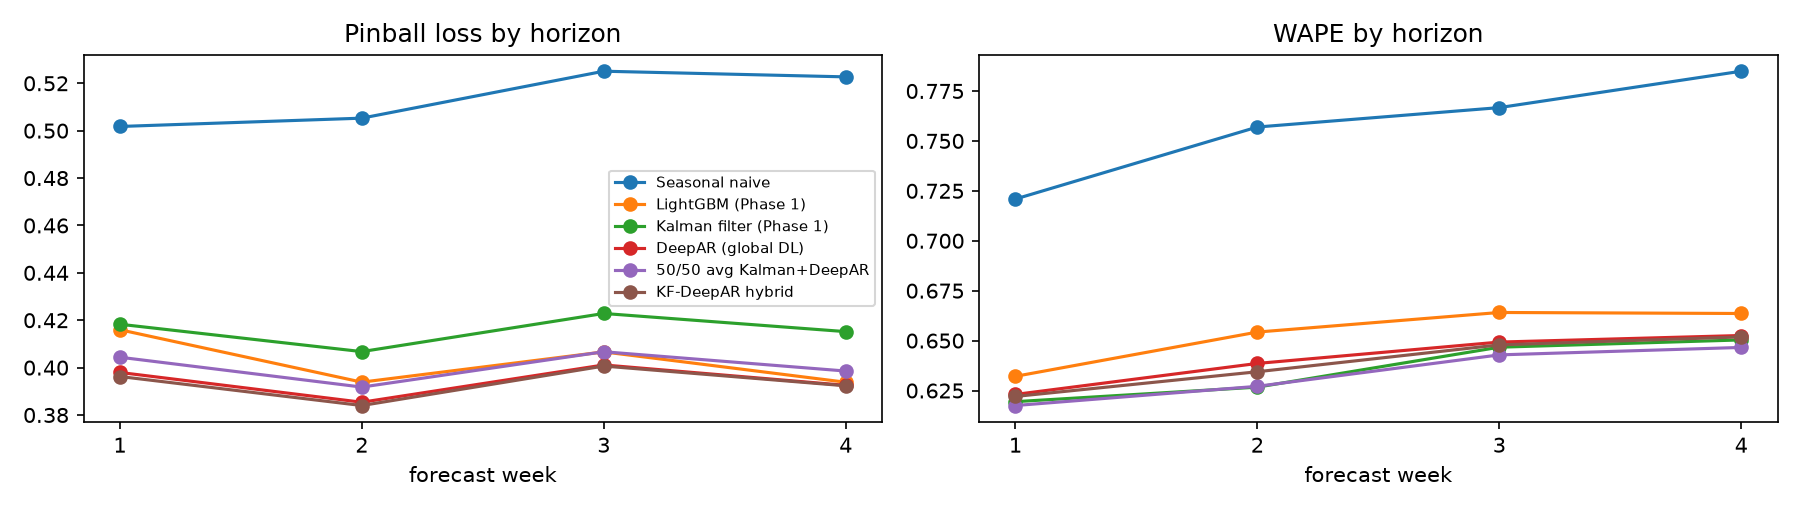
\includegraphics[width=\columnwidth]{06_by_horizon.png}
\caption{Pinball loss and WAPE by forecast week (same horizons for all models).}
\label{fig:horizon}
\end{figure}

\subsection{Demand segments and departments}
Table~\ref{tab:seg} breaks the pinball loss down by demand segment. The deep models gain most on \emph{lumpy} and \emph{intermittent} SKUs
(e.g.\ lumpy: 0.461 vs.\ 0.510 for the Kalman filter, $-9.6\%$), exactly the sparse histories where the local filter cannot learn seasonality
on its own (Section~\ref{sec:gap}). On \emph{smooth} SKUs the Kalman filter is competitive. By department, DeepAR and KF-DeepAR are best for
FOODS\_3 and HOUSEHOLD\_1 and tie with LightGBM on HOBBIES\_1.

\begin{table}[t]
\centering
\caption{Pinball loss by demand segment (DL: mean over seeds).}
\label{tab:seg}
\begin{tabular}{lcccc}
\toprule
Model & smooth & erratic & intermittent & lumpy\\
\midrule
Seasonal naive & 1.090 & 2.003 & 0.287 & 0.624\\
LightGBM & 0.885 & \textbf{1.526} & 0.225 & 0.471\\
Kalman filter & 0.870 & 1.584 & 0.235 & 0.510\\
DeepAR & 0.869 & 1.531 & \textbf{0.220} & \textbf{0.461}\\
50/50 average & \textbf{0.856} & 1.534 & 0.226 & 0.478\\
KF-DeepAR & 0.864 & \textbf{1.526} & \textbf{0.220} & \textbf{0.461}\\
\bottomrule
\end{tabular}
\end{table}

\subsection{The gap that motivates global learning}\label{sec:gap}
To isolate the ``sharing'' limitation of local filters we replaced each SKU's weekday profile by its department-pooled profile.
With the full $\sim$2.5-year history this changes WAPE by less than $\pm1.1\%$; when the profile is estimated from only the last eight weeks,
pooling improves WAPE in \emph{every} segment (smooth $+1.8\%$, intermittent $+1.0\%$, lumpy $+0.9\%$, erratic $+0.3\%$). The information
needed for short or sparse histories lies in other SKUs, which only a global model can use.

\subsection{Uncertainty and stockouts}
The DL models have the narrowest 80\% intervals (3.67--3.68 units vs.\ 3.99 for LightGBM and 4.03 for Kalman) yet the highest empirical coverage
(0.91). This over-coverage is largely an artefact of discrete data: for intermittent SKUs $q_{0.1}=0$, so every zero lies inside the interval.
5.7\% of test cells are flagged as probable stockouts; restricted to in-stock days the ranking is unchanged (KF-DeepAR 0.399, DeepAR 0.400,
50/50 0.403, LightGBM 0.406, Kalman 0.417).

\subsection{Significance}
The paired bootstrap (Table~\ref{tab:sig}) shows that KF-DeepAR is significantly better than seasonal naive, LightGBM, the Kalman filter and the
50/50 average. Its difference to DeepAR is not significant (the CI contains 0). Its seed-to-seed standard deviation of the pinball loss is lower
(0.0011 vs.\ 0.0036), although with three seeds this is indicative rather than conclusive.

\begin{table}[t]
\centering
\caption{Per-SKU pinball difference KF-DeepAR $-$ other model (negative = hybrid better), 95\% bootstrap CI, share of SKUs where the hybrid wins.}
\label{tab:sig}
\begin{tabular}{lccc}
\toprule
vs.\ model & mean diff. & 95\% CI & hybrid wins\\
\midrule
Seasonal naive & $-0.1196$ & $[-0.1404,-0.1006]$ & 94\%\\
LightGBM & $-0.0077$ & $[-0.0128,-0.0030]$ & 65\%\\
Kalman filter & $-0.0217$ & $[-0.0288,-0.0154]$ & 85\%\\
50/50 average & $-0.0063$ & $[-0.0092,-0.0034]$ & 77\%\\
DeepAR & $-0.0005$ & $[-0.0024,+0.0016]$ & 48\%\\
\bottomrule
\end{tabular}
\end{table}

\subsection{Cold start}
Thirty SKUs (10 per department) were removed from training and given only 28 days of history at origin O3; the global models use the
``unknown item'' embedding learned through item-ID dropout. Table~\ref{tab:cold} shows that KF-DeepAR is the best model on every metric.
DeepAR alone knows the department's patterns but not the new SKU's level; the Kalman filter knows the level after a few days but nothing else;
the hybrid combines both.

\begin{table}[t]
\centering
\caption{Cold-start experiment (30 unseen SKUs, 28 days of history, origin O3, seed 0).}
\label{tab:cold}
\begin{tabular}{lccc}
\toprule
Model & MAE & WAPE & Pinball\\
\midrule
Kalman (fitted on 28 days) & 1.747 & 0.615 & 0.571\\
DeepAR (unknown item) & 1.786 & 0.629 & 0.556\\
\textbf{KF-DeepAR (unknown item)} & \textbf{1.739} & \textbf{0.612} & \textbf{0.552}\\
\midrule
\multicolumn{4}{l}{\emph{Reference: same SKUs with full history}}\\
DeepAR & 1.818 & 0.640 & 0.547\\
KF-DeepAR & 1.745 & 0.614 & 0.520\\
\bottomrule
\end{tabular}
\end{table}

\subsection{Ablation study}
Table~\ref{tab:abl} removes one component of KF-DeepAR at a time (3 origins $\times$ 3 seeds; paired by origin and seed).
A change is treated as real only if it exceeds the seed std and has the same sign in most of the nine paired runs.

\begin{table}[t]
\centering
\caption{Ablations of KF-DeepAR (mean over 3 seeds). $\Delta$: change of the pinball loss vs.\ A0; ``worse'': paired runs (of 9) in which the variant is worse than A0.}
\label{tab:abl}
\begin{tabular}{lcccc}
\toprule
Variant & Pinball & $\Delta$ all & $\Delta$ in-stock & worse\\
\midrule
A0 full KF-DeepAR & 0.3941 & -- & -- & --\\
A1 $-$ Kalman channels & 0.3946 & $+0.1\%$ & $+0.2\%$ & 5/9\\
A2 $-$ item embedding & 0.3956 & $+0.4\%$ & $+0.3\%$ & 4/9\\
A3 $-$ calendar \& price & 0.3940 & $-0.0\%$ & $+0.0\%$ & 4/9\\
A4 Gaussian likelihood & 0.4130 & $\mathbf{+4.8\%}$ & $\mathbf{+4.0\%}$ & \textbf{9/9}\\
A5 GRU instead of LSTM & 0.3940 & $-0.0\%$ & $-0.1\%$ & 3/9\\
A6 $-$ regularisation & 0.3936 & $-0.1\%$ & $-0.1\%$ & 5/9\\
A7 $-$ stockout masking & 0.3904 & $-0.9\%$ & $-0.1\%$ & 2/9\\
\bottomrule
\end{tabular}
\end{table}

\begin{figure}[t]
\centering
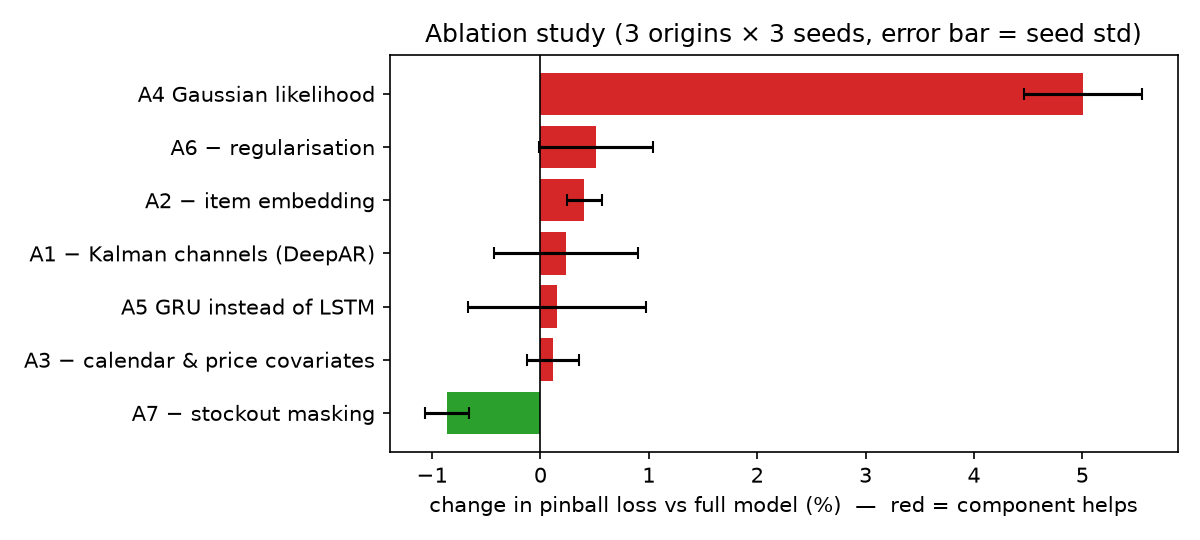
\includegraphics[width=\columnwidth]{05_ablation_bar.png}
\caption{Ablation study; error bars are the seed standard deviation.}
\label{fig:abl}
\end{figure}

\textbf{Likelihood (A4)} is the one clearly important choice: a Gaussian must put probability on negative sales and cannot represent the
spike at zero, so it is worse in all nine runs (coverage drops to 0.87 with wider, mis-shaped intervals).
\textbf{Kalman channels (A1), item embedding (A2), covariates (A3), GRU (A5) and regularisation (A6)} change the loss by less than $0.4\%$,
within seed noise. For A6 the train/validation curves explain why: with 27.6k parameters, random windows and early stopping, the model does not
over-fit (validation NLL stays below training NLL in both settings), so extra regularisation has little to do. The covariates are largely
redundant with the 56-day context, from which the LSTM can infer the weekly cycle.
\textbf{Stockout masking (A7)} looks harmful on \emph{all} days ($-0.9\%$) but is neutral on in-stock days ($-0.1\%$): a model that learns from
stockout zeros predicts lower values and is rewarded on the 5.7\% of test days that are themselves stockouts. Those zeros are censored demand,
so the in-stock column is the relevant one for inventory planning; masking does not hurt there and keeps the forecast an estimate of
\emph{demand} rather than of \emph{sales}.


%======================================================================
\section{Discussion}
\textbf{Local vs.\ global.} The Kalman filter remains a strong point forecaster: with long histories its level estimate is hard to beat, and it
handles stockouts as missing data exactly. Its weakness is the forecast \emph{distribution} and sparse series. The global DL model learns shared
patterns and a count likelihood, which pays off in the pinball loss, especially for lumpy and intermittent SKUs.

\textbf{Is the hybrid meaningful?} It is technically justified (causal, uses the optimal local state summary, follows the ES-RNN/DSSM line of
work), it is significantly better than the naive ML+DL average, it varied less across seeds and it is the best model for cold-start SKUs.
The ablation confirms that, for SKUs with long histories, removing the Kalman channels changes the loss by only $0.1\%$.
Its average gain over DeepAR is small because most fitted filters are very smooth (median $q/r\approx6\cdot10^{-4}$): for long histories the Kalman
level is close to the context mean that DeepAR already receives through $\nu$. The Kalman channels matter where local information is scarce.

\textbf{What the ablations teach.} On this data the \emph{likelihood} matters far more than architecture details (LSTM vs.\ GRU) or
regularisation strength; small single-seed differences between deep-learning variants should not be trusted.

\textbf{Limitations.} One store and 300 SKUs; the stockout detector is a heuristic (it flags 8.6\% of days and may flag some genuine zero-demand
runs); hyper-parameters follow the DeepAR paper and were not tuned; the cold-start experiment uses one origin and one seed; interval coverage of
count forecasts is inflated by discreteness (a randomised PIT would be a better calibration check).

%======================================================================
\section{Conclusion and Future Work}
We built a leak-free DL pipeline for retail demand, a from-scratch DeepAR and a Kalman-informed hybrid, and compared them with the Phase-1 models
under one rolling-origin protocol with probabilistic metrics, seed variance, significance tests, a cold-start study and ablations. Global deep
learning improves the probabilistic accuracy over both local and tabular baselines, the count likelihood is the most important design
choice, and feeding the local Kalman state to the network helps most where local history is scarce (cold start). Future work: let the network output the Kalman noise parameters per SKU and day (a deep state-space model
\cite{rangapuram2018dssm}), replace the LSTM by attention (TFT~\cite{lim2021tft}) or a selective SSM (Mamba~\cite{gu2023mamba}), and tune the
stockout threshold.

\appendices
\section{Individual Contributions}
Roles were assigned at random. Each member owns one notebook, one section of the shared library notebook and one part of this report.
\begin{table}[h]
\centering
\caption{Contributions.}
\begin{tabular}{p{1.7cm}p{6.0cm}}
\toprule
Member & Work\\
\midrule
Saumya & Data pipeline, causal stockout detector, features, segments, DL window sampler (nb.~01; lib.~B; Sec.~III)\\
Harshvardhan & Kalman filter from scratch with MLE, Phase-1 baselines, gap analysis (nb.~02; lib.~C; Sec.~IV-A/B)\\
Shivansh & DeepAR network, NB likelihood, training and sampling, embeddings (nb.~03; lib.~D; Sec.~IV-C/E)\\
Krishiv & KF-DeepAR hybrid, 50/50 control, cold-start experiment (nb.~04; lib.~E; Sec.~IV-D, VI-G)\\
Harsha & Evaluation protocol and metrics, ablations, significance tests (nb.~05--06; lib.~A,F; Sec.~V--VI)\\
\bottomrule
\end{tabular}
\end{table}


\bibliographystyle{IEEEtran}
\bibliography{references}

\end{document}
